%%
%%  Department of Electrical, Electronic and Computer Engineering.
%%  EPR400/2 Final Report - Section 2.
%%  Copyright (C) 2011-2021 University of Pretoria.
%%

\section{Approach}
The aim of this project was to develop a system that would illuminate flying mosquitoes with a laser turret. Throughout the remainder of this document this system will be referred to as the \gls{mads}. The project can be viewed in terms of a set of integrated subsystems. The subsystems are as follows:
\begin{description}[style=nextline]
      \item[Laser Turret Control System] This subsystem is responsible for controlling the laser turret. The laser control system is discussed in
            % \autoref{sec:laser_turret_control_system}.
      \item[Laser Detection System] This subsystem is responsible for detecting the actual position of the laser with the camera. The laser detection is required to provide feedback to the laser turret control system. The laser detection system is discussed in
            % \autoref{sec:laser_detection_system}.
      \item[Mosquito Detection System] This subsystem is responsible for detecting the position of the mosquitoes. The mosquito detection system is discussed in
            % \autoref{sec:mosquito_detection_system}.
      \item[Mosquito Tracking System] This subsystem is responsible for tracking the mosquitoes and predicting their future positions. The mosquito tracking system is discussed in
            % \autoref{sec:mosquito_tracking_system}.
\end{description}

The subsystems were integrated on a real-time embedded system and will be discussed in detail in the relevant sections. The system is designed to operate in a controlled environment constructed specifically for this project. The functional block diagram of the \gls{mads} is shown in \autoref{fig:functional_block_diagram}.

\begin{figure}[h]
      \centering
      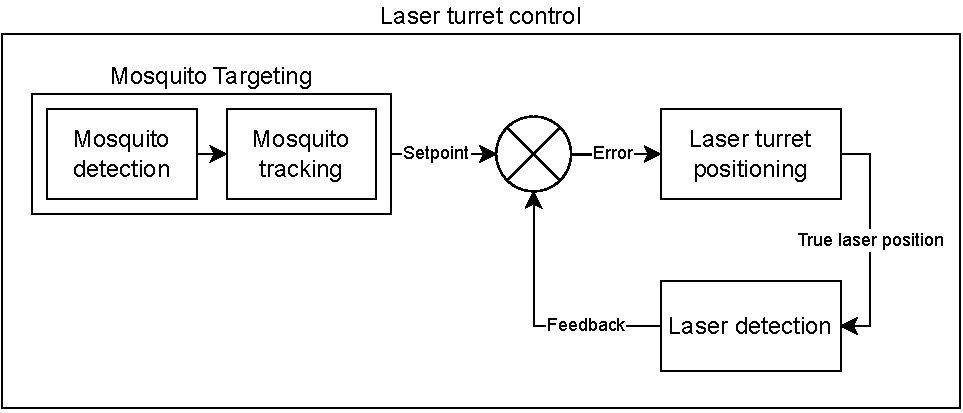
\includegraphics[width=1\textwidth]{figures/function_block_diagram.drawio.pdf}
      \caption{Functional block diagram of the \gls{mads}.}
      \label{fig:functional_block_diagram}
\end{figure}

The design choices for the \gls{mads} were made with careful consideration of the implicit real-time operation requirement of the system. All aspects of the \gls{mads} were designed to be as lightweight as possible in terms of computational complexity.

\newpage

%% End of File.

